\documentclass[a4 paper]{article}

\usepackage{amsmath, amsthm, amsfonts} 
\usepackage[skip = 10pt, indent = 30pt]{parskip}    
\usepackage{setspace}
\onehalfspacing
\usepackage{caption}
\usepackage{subcaption}
\usepackage{pdfpages}\usepackage{booktabs}
\usepackage{textcomp}
\usepackage{amssymb}
\usepackage[document]{ragged2e}
\usepackage{bm}
\usepackage[brazil]{babel}
\usepackage[backend=biber,style=numeric]{biblatex}
\addbibresource{biblio.bib}
\usepackage{tcolorbox}
\usepackage{changepage} 


\newcommand{\parag}{\hspace{30pt}}


\title{TAC - Seizure Recognition}
\author{Yuri Shumyatsky - 231012826\\Gabriel Gonçalves Caldo - 231034627\\Pedro Araujo Cordeiro Viana - 202067452}
\date{\today}
\begin{document}

\maketitle
\newpage

\section{Introdução}
\parag O objetivo do projeto é a simulação e planejamento de uma missão robótica, retirada especialmente do repositório RoboMax \cite{robomax}. A escolhida foi a Seizure Recognition, em que um robô deve monitorar um paciente e alertar uma central caso o paciente sofra uma convulsão. O texto dos requisitos dessa missão é o seguinte:

\begin{adjustwidth}{-3cm}{-3cm}
\begin{center}
\begin{tcolorbox}[width=14.5cm]
The robot is located in the patients room. It will observe the patient and start interacting, if the patient seems to be non responsive or presents repetitive movements. Further triggers for interaction are provided by sensors and seizures detection software from EEG. When triggered, a robot should check attention and responsiveness of a patient. The robot must start the task within 30-60 seconds. In case of not being able to do so, a nurse should be immediately alerted. In order to be able to perform this task on very short notice, the robot should be within the patient room or very close by. At the time, the task is assigned, the robot should check if all the necessary equipment to collect the required tasks are available in the room, if not, the robot should go to the storage room and collect the equipment (sensors). Battery recharge routines must not be triggered during operating the task. If the robot achieves less than 10\% of battery, it should save checkpoints for every atomic action, log it, and alert the manager of the site. The goal is to improve diagnostic value of seizure reporting by recognising seizures and ictal testing. For diagnostic purposes patient with epilepsy may undergo long term (24/7) video EEG monitoring for several days in hospital. Aim is to record seizures simultaneously on EEG and video. For the reporting of such seizure recordings it is important to know, if the patient is aware and responding, or if any of these capabilities is impaired. Therefore, applying a standardized test sequence of verbal commands and showing pictures to the patient as well as recording and interpreting the responses is crucial. A significant increase of heart rate is present in approx. 80\% of focal epileptic seizures. At the same time, EEG changes occur and the patient's behaviour changes (e.g behavioural freezing, repetitive stereotyped movements, or non responsiveness). The robot will follow and observe the patient and will assess data provided by the Video-EEG analysis/seizure detection software or sensors (e.g., movement pattern detection and/or heart rate). If a heart rate increase occurs, the seizure detection software alerts, or the patients behavior changes, the robot will start to interact with the patient. Initially, it will ask if the patient is well or experiences a seizure. If there is no response or the patient confirms a seizure, the robot will start to apply the test sequence to the patient and alert the nurses to attend. The task is completed when a stop signal is received or a certain amount of time (specified beforehand) has passed. 
\end{tcolorbox}
\end{center}
\end{adjustwidth}

\section{MutRoSe - iHTN's}
\parag Dada a escolha da missão como sendo a Seizure Recognition do repositório RoboMax \cite{robomax}, foi utilizado a extensão do VSCode para o uso do MutRoSe e para a decomposição da missão e elaboração das iHTN's. 

\begin{table}[h]
\centering
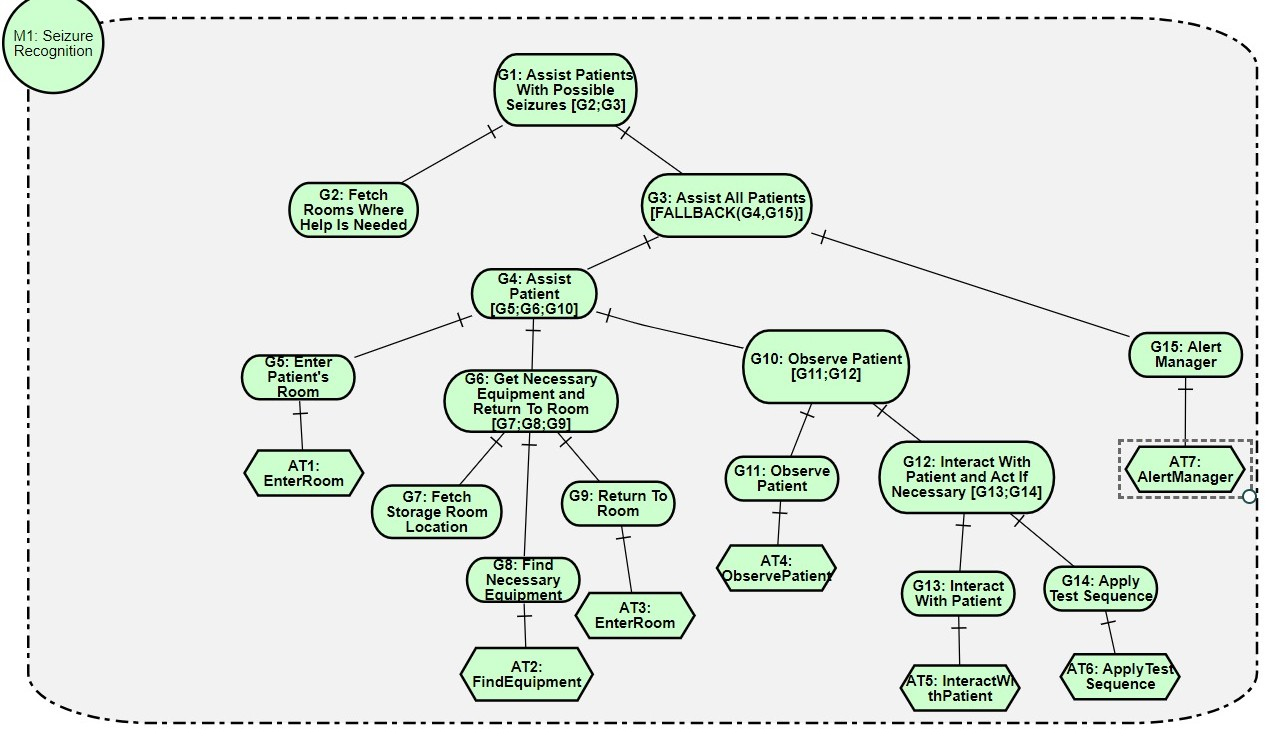
\includegraphics[scale=0.3]{figuras/gm}
\end{table}
\begin{center}
Figura 1: Goal Model da Missão
\end{center}
\vspace{15pt}

Ao decompor essa missão, foram geradas inúmeras iHTNs (em torno de 1340), mas foi selecionada a iHTN de número $666$ para basear a construção da Behavior Tree.
\vspace{15pt}\vspace{15pt}

\begin{table}[h]
\centering
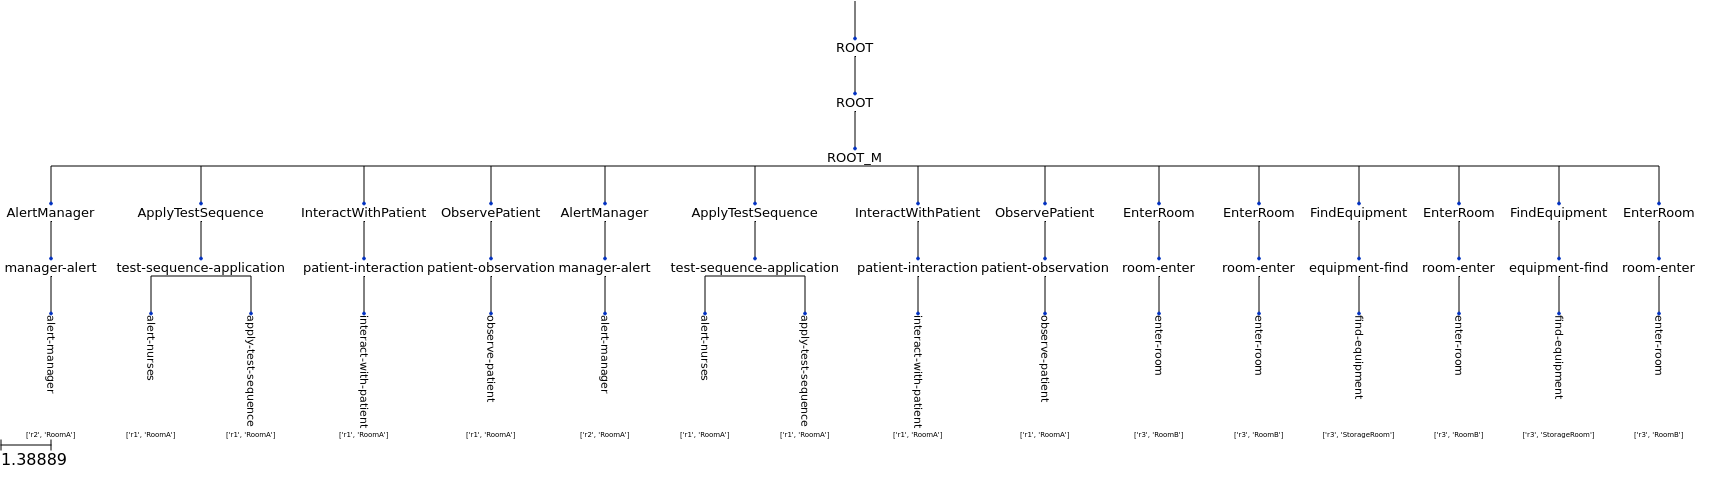
\includegraphics[scale=0.25]{figuras/ihtn_666}
\end{table}
\begin{center}
Figura 2: iHTN 666
\end{center}
\vspace{30pt}

O resultado é portanto a Behavior Tree da Figura 3.

\newpage
\begin{table}[h]
\centering
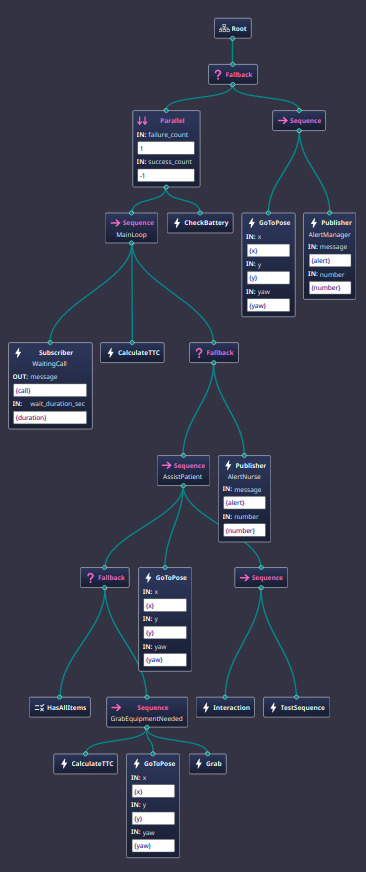
\includegraphics[scale=0.5]{figuras/bt}
\end{table}
\begin{center}
Figura 3: BT simulada no Groot
\end{center}

\section{Configuração do Mapa}
\parag Apesar dos arquivos para o mapa do hospital terem sido providenciados, foram gastas múltiplas horas tentando fazer com que a simulação usasse os arquivos corretos, mas não houve sucesso. 

De fato,  o mais próximo alcançado foi a presença apenas das paredes, sem texturas ou objetos, como mostra a Figura 4.

%Figura 4

Além disso, foi testado também com o mapa do CiC, mas não houve sucesso.


\begin{table}[h]
\centering
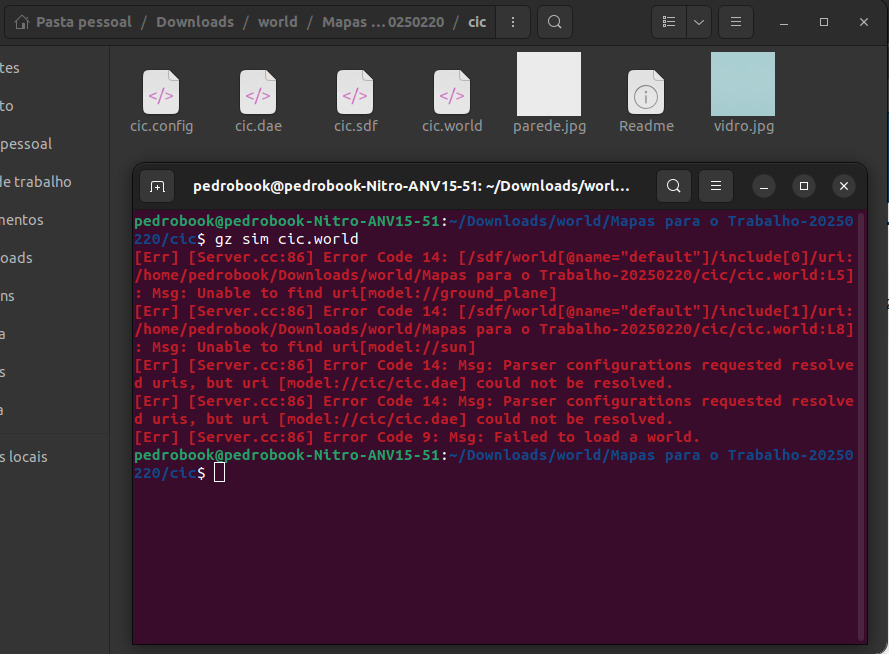
\includegraphics[scale=0.4]{figuras/cicerror}
\end{table}
\begin{center}
Figura 5: Erro ao usar o mapa CiC
\end{center}

\section{Build}
\parag Ao tentar usar o CMake para organizar os arquivos e construir um binário, ocorreram erros que impediram a execução da Behavior Tree. 

Principalmente, um erro foi o não reconhecimento dos ports do nó de controle "Paralelo", apesar do nó ser o padrão do programa Groot 2. 




\section{Conclusão}
\end{document}
